% $Id: template.tex 11 2007-04-03 22:25:53Z jpeltier $

\documentclass{vgtc}                          % final (conference style)
%\documentclass[review]{vgtc}                 % review
%\documentclass[widereview]{vgtc}             % wide-spaced review
%\documentclass[preprint]{vgtc}               % preprint
%\documentclass[electronic]{vgtc}             % electronic version

%% Uncomment one of the lines above depending on where your paper is
%% in the conference process. ``review'' and ``widereview'' are for review
%% submission, ``preprint'' is for pre-publication, and the final version
%% doesn't use a specific qualifier. Further, ``electronic'' includes
%% hyperreferences for more convenient online viewing.

%% Please use one of the ``review'' options in combination with the
%% assigned online id (see below) ONLY if your paper uses a double blind
%% review process. Some conferences, like IEEE Vis and InfoVis, have NOT
%% in the past.

%% Figures should be in CMYK or Grey scale format, otherwise, colour 
%% shifting may occur during the printing process.

%% These three lines bring in essential packages: ``mathptmx'' for Type 1 
%% typefaces, ``graphicx'' for inclusion of EPS figures. and ``times''
%% for proper handling of the times font family.
\usepackage{lmodern}
\usepackage{subfig}
\usepackage{amsmath}
\usepackage{amssymb}
\usepackage{mathptmx}
\usepackage{graphicx}
\usepackage{times}
\usepackage{url}
\usepackage{enumitem}
\usepackage{algorithm}
\usepackage{array}
\usepackage[pdftex]{adjustbox}

%% We encourage the use of mathptmx for consistent usage of times font
%% throughout the proceedings. However, if you encounter conflicts
%% with other math-related packages, you may want to disable it.

%% If you are submitting a paper to a conference for review with a double
%% blind reviewing process, please replace the value ``0'' below with your
%% OnlineID. Otherwise, you may safely leave it at ``0''.
%\onlineid{1703}
\onlineid{0}

%% declare the category of your paper, only shown in review mode
\vgtccategory{Research}

%% allow for this line if you want the electronic option to work properly
\vgtcinsertpkg

%% In preprint mode you may define your own headline.
%\preprinttext{To appear in an IEEE VGTC sponsored conference.}

%% Paper title.

\title{Visual Analysis of Body Movement for Healthcare}

%% This is how authors are specified in the conference style

%% Author and Affiliation (single author).
%%\author{Roy G. Biv\thanks{e-mail: roy.g.biv@aol.com}}
%%\affiliation{\scriptsize Allied Widgets Research}

%% Author and Affiliation (multiple authors with single affiliations).
%%\author{Roy G. Biv\thanks{e-mail: roy.g.biv@aol.com} %
%%\and Ed Grimley\thanks{e-mail:ed.grimley@aol.com} %
%%\and Martha Stewart\thanks{e-mail:martha.stewart@marthastewart.com}}
%%\affiliation{\scriptsize Martha Stewart Enterprises \\ Microsoft Research}

%% Author and Affiliation (multiple authors with multiple affiliations)
\author{Oky Purwantiningsih\thanks{e-mail: oky.purwantiningsih@lirmm.fr}\\ %
        \parbox{2in}{\scriptsize \centering LIRMM \\ Universit\'{e} Paul Val\'{e}ry Montpellier} %
\and Arnaud Sallaberry\thanks{e-mail: arnaud.sallaberry@lirmm.fr}\\ %
     \parbox{2in}{\scriptsize \centering LIRMM \\ Universit\'{e} Paul Val\'{e}ry Montpellier} \\  \\ %
\and S\'{e}bastien Andary\thanks{e-mail: sebastien@naturalpad.fr}\\ %
\parbox{2in}{\scriptsize \centering NaturalPad}%
\and Antoine Seilles\thanks{e-mail: antoine@naturalpad.fr}\\ %
\parbox{2in}{\scriptsize \centering NaturalPad}%
\and Jer\^{o}m\'{e} Az\'{e}\thanks{e-mail: jerome.aze@lirmm.fr}\\ %
\parbox{2in}{\scriptsize \centering LIRMM \\ Universit\'{e} de Montpellier} %
	} %


%% A teaser figure can be included as follows, but is not recommended since
%% the space is now taken up by a full width abstract.
%\teaser{
%  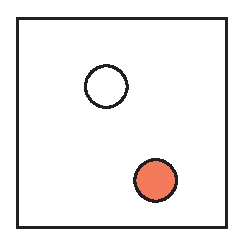
\includegraphics[width=1.5in]{sample.eps}
%  \caption{Lookit! Lookit!}
%}

%% Abstract section.
\abstract{The advancement of motion sensing input devices has enabled the collection of  multivariate time series body movement data. Analysing such type of data is a challenge due to the large amount of data generated as well as in finding interesting movement pattern overtime. To address this problem, we propose a visualization interface to analyse body movement data. We propose two views: (i) Session View, which allows movement analysis on a particular time point (ii) Summary View which allows analysis of movement overtime. This view enables users to navigate and explore the evolution of movement overtime for different movement area. Here we propose a clustering method based on hierarchical clustering to group similar movement pattern. The proposed visualization is illustrated with a case study which demonstrate the ability of the interface to analyse body movement.
} % end of abstract

%% ACM Computing Classification System (CCS). 
%% See <http://www.acm.org/class/1998/> for details.
%% The ``\CCScat'' command takes four arguments.

\CCScatlist{ 
  \CCScat{H.3.3}{Information Storage and Retrieval}%
{Information Search and Retrieval}{Clustering};
  \CCScat{H.5.2}{Information Interfaces and Presentation}{User Interfaces}{Graphical User Interfaces}
}

%% Copyright space is enabled by default as required by guidelines.
%% It is disabled by the 'review' option or via the following command:
% \nocopyrightspace

%%%%%%%%%%%%%%%%%%%%%%%%%%%%%%%%%%%%%%%%%%%%%%%%%%%%%%%%%%%%%%%%
%%%%%%%%%%%%%%%%%%%%%% START OF THE PAPER %%%%%%%%%%%%%%%%%%%%%%
%%%%%%%%%%%%%%%%%%%%%%%%%%%%%%%%%%%%%%%%%%%%%%%%%%%%%%%%%%%%%%%%%

\begin{document}

%% The ``\maketitle'' command must be the first command after the
%% ``\begin{document}'' command. It prepares and prints the title block.

%% the only exception to this rule is the \firstsection command
\firstsection{Introduction}

\maketitle

%% \section{Introduction} 

Visualizing movement data has been proved to be a challenge due to its large volume \cite{adrienko_book}. This is also the case with visualizing body movement data which is usually multivariate and time oriented. The challenge in visualizing time-series data lies in finding the temporal trends or pattern in the data as has been discussed extensively in \cite{aigner}. Unfortunately there has been very few visualization technique which focus on time-series body movement data (for example \cite{bernard2013}). In healthcare, such data are generated from serious game which are used for patients' rehabilitation and training. These games use motion sensing input device technologies such as Kinect and Wii Balance Board to capture players' movement. The data generated from the game are then analysed by healthcare professionals to make diagnostic of patients' progress. However, analysing large amount of data manually is long, difficult and tedious. Hence, a visualization interface is needed. The challenge lies on how to visualize such data so that healthcare professionals can evaluate the rehabilitation progress and make decision for the next step of the process.

Currently, serious games provide some charts which visualize player's body movement with respect to the horizontal axis and vertical axis. However, the information that can be gathered from the visualization is not enough for the healthcare professional to establish an informed diagnostic. It's hard to know how often the player move to the right or left. It's also not possible to know to which type of events (ie. avoiding an enemy, catching the bonuses) the movement is related. Which is crucial since the therapist need to know if the player is able to move his body to the right direction. Most importantly, they need to know evolution of players' body movement overtime to see if they have developed strategy to circumvent the movement required for the rehabilitation.

To address these problems, we proposed a visualization interface for healthcare professionals to visualize the gameplay data to help them analyse patients' movement during the game as part of rehabilitation process. The visualization provides two type of visualizations: (1) visualization which provides information on frequency and direction of body movements which are related to objects in the game for one game session. (2) An interactive visualization where healthcare professionals can analyse the evolution of player's body movement throughout all sessions. Here, we proposed an approach to easily navigate and highlight movement pattern. We also proposed a clustering algorithm based on hierarchical clustering to identify similar movement pattern. A distance function is defined to quantify movement pattern similarity which consider both movement evolution and proportion of movement frequency.

The remainder of this paper is organized as follows. Section 2 discuss the domain problem characterization. Section 3 explores related work. The data abstraction is presented in Section 4. The Visual Mapping and Interactive Functionalities of the proposed visualization are discussed in details in Section 5. Section 6 provides a case study used to evaluate the approaches and finally, Section 7 concludes the paper.

\section{Domain Problem Characterization}

In order to clearly understand the problems faced by the healthcare professional in interpreting a gameplay into a meaningful therapy routine, it is important to have an understanding of how the game is played. Based on this understanding, then it will be possible to find out what kind of information is needed by defining questions usually asked by the users. In the end, visualization requirement elicitation will be done by translating each question into list of tasks. This section discusses each one of these steps in details.

For the research, we explore data from a game called Hammer and Planks which is developed by NaturalPad\footnote{\url{www.naturalpad.fr}}. It is designed to train and rehabilitate hemiplegic patient. A person with hemiplegic is paralyzed on one side of the body. Therefore, the gameplay is designed so that the player has to move his body to the right, left, forward and backward in order to train their affected side of the body. Hammer and Planks is a vertical shooter game. The game world is in a 2D environment vertically scrolling from top to bottom in which a player navigate a ship from left to right through moving his body. While navigating the ship to collect driftwood/plank (bonuses), the player also needs to kill enemies and avoiding reefs scattered all over the ocean (obstacles).

Played with Kinect, it is possible to play Hammer and Planks in two different ways: (i) BodyTilt: Player puts both arms in his/her hips and move the upper body (from the waist up) to the right, left, forward or backward to navigate the boat. (ii) HandPoint: Player lifts one of his/her forearm in front of the body with the palm facing forward. Navigating the boat can be done by moving the forearm to the right, left, forward, or backward. Basically, there are two type of movement directions: horizontal movement moves the boat horizontally and Vertical movement changes boat speed.

Before each session, the healthcare professionals will set the number of objects (enemies, bonuses, obstacles), activity duration and repetition, as well as area in which the objects can appear. Therefore he can adjust the difficulty of the game for different session.

\subsection{Target User Questions}

A traditional Hemiplegic therapy routine usually involved the therapist ordering a patient to perform several movement repetitively \cite{rahman}. By the end of the session, the therapist will analyse how the patient has performed based on the quality of movement as well as how the patient has progressed compared to the previous session. Based on this analysis, the therapist will then configure a new routine to further the patient's progress, if needed.

However, by using a game to facilitate the therapy, it is difficult to monitor how often the patient has moved his/her arm, to which direction and to which objects this movement is associated. Based on these reasons, we identified 5 types of questions usually inquired: (Q1) For a given session, to which direction (right/left) the player moved more? (Q2) For a given session, how does the player perform based on the number of objects collected, avoided, or killed with respect to the area of the movement? (Q3) For a given session, how does the player perform based on the number of objects collected, avoided, or killed with respect to the area of movement and the speed in which the game is played? (Q4) For a given patient, has he/she improved in the game overtime?(Q5) For a given patient, has he/she improved in a certain area overtime?

\subsection{Visualization Requirements}

The gameplay of each game session contains information of the player, game setting, player movement throughout the game and every events happened in the game. Each event has an event type, which is the type of action performed by a player (represented with a boat in the game) towards an object or the other way around. Based on these information and the question defined in the previous section, the visualization tasks can be grouped into: task related to a session for a particular player (\textit{T}1) and task related to the summary of all sessions for a player (\textit{T}2). The following are the tasks defined for each task group:
\newcommand{\task}[2]{$#1 #2$}
\begin{enumerate}[label=\textbf{(\task{T1.}{\arabic*})}]
\item \label{t11} Visualize and be able to compare the number of events within the same or among different event type at a given x area (Q1,Q2).
\item \label{t12} Visualize and be able to compare the number of events and its screen speed of the same or among different event type at a given x area (Q1,Q2,Q3).
\item \label{t13} Select and visualize the number of events for a certain object at a given x area (Q1,Q2).
\item \label{t14} Select and visualize the number of events and its screen speed for a certain object at a given x area (Q1,Q2,Q3).
\end{enumerate}

\newcommand{\test}[2]{$#1 #2$}
\begin{enumerate}[label=\textbf{(\test{T2.}{\arabic*})}]
\item \label{t21} Visualize, navigate and be able to compare the evolution of number of events throughout all sessions within a certain x area (Q4,Q5).
\item \label{t22} Select and visualize the number of events of a certain event type in a certain x area throughout all sessions (Q4,Q5).
\item \label{t23} Visualize, navigate and be able to compare the distribution of a certain number of events over x area among all sessions (Q4,Q5).
\item \label{t24} Select and visualize the distribution of certain number of events over x area for a certain event type throughout all sessions (Q4,Q5).
\item \label{t25} Extract and visualize similar pattern of number of events evolution throughout all sessions over a certain x area (Q4,Q5).
\end{enumerate}
\section{Related Works}
There have been several serious game for hemiplegic rehabilitation developed in the last few years. Similar to Hammer and Planks, these games also have some visualization feature which shows how the player performed so that the therapist is able to make the correct diagnosis. Thus, in this section, we first review some of these visualization. Then, since the nature of the input data is time series and movement data, we present some work in visualization which are related to this type of data.

\subsection{Visualization of Serious Game Result} 

Game result visualization is an integral part of a serious game used for rehabilitation since it's the feature which influence the accuracy of therapist analysis. Most serious game have an analytic feature, however the type of analysis presented depends on the nature of the game and the framework used in the rehabilitation. We only focus on reviewing serious game which are directed to hemiplegic patients rehabilitation.

\cite{rahman} present a rehabilitation framework for hemiplegic patients which combines the use of Kinect and LEAP\footnote{\url{https://www.leapmotion.com/product/desktop}} hand-tracking devices. These devices are attached to a 3D based game environment which was set to accommodate a set of primitive therapy motion such as forearm pronation/supination, shoulder and hip joint adduction/abduction, etc. Similar to Hammer and Planks, one of the game used in the framework requires user to navigate a plane by moving the hand to the right and left (hand-elbow flexion-extension). The recorded movement is then presented in line chart depicting the range of axis of elbow joint (180 degrees when fully extended and 20 degrees when fully flexed) over number of frames captured. Similarly, current visualization in Hammer and Planks also uses line chart to show average body movement over time. 

Similar to Hammer and Planks, \cite{rahman2} introduced a framework which uses Kinect attached to Second Life serious game environment. The mission of the game is to follow a set of movement that have been configured beforehand by the therapist. During the game, the movement of each body joint  is recorded and saved in Session Recorder. Afterwards, a Kinematic Analytic component will process this data and visualize the quality of improvement metrics of each body joint movement. Each metric is visualized with a dotted line chart over time. Even though it's possible to  see an elbow flexion or extension from the line curve, the therapist needs to count the number of the curve manually. This is not very efficient when the session is longer and there are more curve to count.

\subsection{Visualization of Time Series Data}

Since one of the requirement of the interface is to have the information of movement evolution over time, it is interesting to review how time series data is usually visualized. Tominski and Aigner discuss at length about the techniques of time series data visualization in their book \cite{aigner}. The visual survey of this book can be found on their website\footnote{\url{http://survey.timeviz.net}}. This section reviews some of these interesting techniques.

Considering that the recorded gameplay data contains spatial information (location of an event happened on the screen), we reviewed techniques which concern visualizing spatio-temporal data. \textbf{Flow Map} \cite{adrienko} depicts movements of object over time. Object movements are usually represented by directed trajectories over spatial space (i.e: map) with different color, width, angle of trajectories represent additional information. In order to overcome overlapping trajectories for huge amount of data, usually aggregation techniques (clustering, self organizing map, etc.) are introduced to group similar data point. Another visualization technique worth to mention is \textbf{Spatio-Temporal Event Visualization} \cite{turdukulov, tominski, gatalsky} which uses the space-time cube concept. In this concept, the x and y axis usually represent two spatial dimensions while the third axis represents temporal dimension. The events are then represented as graphical objects which are mapped to the space-time cube location. Different events attribute can be represented in different size, colors, shape, or texture. Even though space-time cube can portrays the spatio-temporal data, it has some downside. When there are too many events, occlusion is inevitable. It should be coupled with an appropriate interaction technique to allow users see the data from different perspective.

One example of time-series visualization technique which doesn't concern spatial data is \textbf{Theme River}. First introduced in \cite{havre}, Theme River is used to visualize thematic changes over time of document collection. Each theme is represented as different colors which flows from left to right with different width over different time point. The width depicts theme strength over temporal axis. The purpose of this technique was to easily understand the evolution of theme strength over time. By following the flow of a certain color (theme) we can easily see the changes in theme strength and associate it with the events that affects the changes. Theme River should be supported with interaction techniques which allow user to rearrange river positioning over horizontal axis. 

\subsection{Visualization of Movement Data}

Movement data usually represents an object which moves over a certain space \cite{adrienko_book}: data of moving car, birds migration, etc. It's usually recorded as series of location (latitude/longitude, x/y coordinates, etc.) and time. On the other hand, body movement data are recorded as vector representation of human pose \cite{bernard2013} over time. On this subsection, we first review visualization for movement data in general and then discuss visualization for body movement focusing on visualization for skeleton animation data.

There have been numerous method and application developed to analyse movement data. \cite{adrienko} gives an overview on these methods and applications. Movement data for discrete entities are usually represented as linear symbol over a map or space time cube. However, this technique has problem with occlusions for huge amount of data. Therefore, it's usually accompanied with other graph such as time graph. Other solution to this problem is to use clustering on the trajectories. Apart from minimizing the number of trajectories presented on the view at the same time, clustering also help user to find interesting pattern of the movement. Patterns can also be found by introducing aggregation and generalisation technique on spatial or temporal properties of the movement. For example, the movement data can be aggregated spatially into a discrete grid and for each grid, the number of movement (total or average) happened within the grid can be represented with color or objects in different size. 

Recognizing and understanding human movement has many benefits in different application domain: arts \cite{heryadi,raptis}, sports \cite{bernard2013}, healthcare \cite{patsadu}, etc. There are numerous research have been done concerning human movement analysis as discussed in  \cite{gavrila} which surveyed different methodologies and approaches. Most of the methodologies discussed focus on identifying a certain type of movement. On the other hand, to our knowledge, there hasn't been many research which focus on human body movement visualization in which user can explore and analyse a certain data set. 

\cite{chmelik} proposes a system to track and visualize body movement on a virtual environment in real time. In this system, body parts  which desired to be tracked are attached to an optical system with twelve infrared cameras. Once user move the tracked body parts, a "motion trail" will be shown in the virtual environment in which then user can manipulate its representation by changing the color, shape, smoothness, etc. These interaction also conducted directly in the virtual environment. 

Another approach to visualize body movement is by using color belt \cite{yuko}. In this approach, movement data collected from motion capture system with 11 sensors attached in body joints are grouped into 4 limbs movement: Right Arm, Left Arm, Right Leg, Left Leg. Each of the limb representation is arranged in vertical axis sequentially forming a belt. The horizontal axis represents time (from left to right) and the sections represent sets of movement. Limb motions are shown as gradation of red-green colors in this belt by extracting the position and angle of associated body joints data. Positive angle is represented with red color, while negative angle is represented with green color.

MotionExplorer \cite{bernard2013} introduced human motion exploratory search using hierarchical aggregation. This approach are directed towards the need to explore huge quantity of motion data and be able to identify interesting sequence of movements. Implemented on database which contains various motions in multiple repetitions, first each human pose data is clustered using k-means algorithm. A pose cluster comprises of a large numbers of similar human pose and is represented as a circular glyph with human stick-figure pose as the centroid and set of pose in the cluster as deviating, transparent figures. The cycle around cluster glyph are colored based on color legend and shows similarity among clusters. With MotionExplorer, user can explore all available pose cluster hierarchically, shows sequences between pose clusters, and search for a specific motion sequence.

\section{Data Abstraction}
In this section we discuss the design of data structure and clustering technique used to support the visualization requirement. First, an overview of the input data generated from the game will be explained. Then a description on how this data is extracted to be the input of the visualization interface will be given. Finally, a clustering algorithm proposed to be used in the visualization will be discussed.

\subsection{Game Event Structure}
\subsubsection{Event Category}
The goal of Hammer and Planks game is to kill all of the enemies while avoiding any attack from the enemies and obstacles \cite{diloreto}. Along the way, player can also catch bonuses to increase their score. Based on these, we identified three different objects within the game: Enemy, Bonus, and Obstacle. For each of these object, there are certain events associated. Each event has an event type. In total, there are 7 event types: (1) Catch: when a bonus is catched (2) Miss: when a bonus is missed or player's attack on enemy is missed (3) Dodge: when an obstacle is avoided (4) Collision: when the player's boat collide with an enemy or obstacle (5) Kill: when an enemy is destroyed by player's boat (6) Hit: when the player's attack hit an enemy (7) Hurt: when the enemy's attack hit player's boat.

Based on the level of impact of each event to the user's boat, we characterize the event by assigning it with Positive, Neutral, or Negative as shown in Table \ref{tblEventType}.
\begin{table}[h]
\begin{center}
    \begin{tabular}{| l | l | l | l |}
    \hline
    Event Type & Bonus & Obstacle & Enemy \\ \hline\hline
    \textbf{Positive} & catch & - & kill,hit\\ \hline
    \textbf{Neutral} & miss & dodge & miss\\ \hline
    \textbf{Negative} & - & collision & hurt, collision\\
    \hline
    \end{tabular}
    \caption {Event Type grouping}
    \label{tblEventType}
\end{center}
\end{table}

\subsubsection{Screen Speed}
Each object and event in the game are assigned with 2D location coordinates (\textit{x},\textit{y}). An \textit{x} axis of this coordinate indicates horizontal axis of the screen. Zero \textit{x} axis is in the middle of the screen. \textit{y} axis indicates vertical axis of the screen. Zero \textit{y} axis is in the middle of the height of the screen, thus -\textit{y} is a location on the lower half of the screen and +\textit{y} is a location on the upper half of the screen.

In the game, a big number of positive events indicate a good player's performance. However, it is important to consider whether the events happened when the player's boat move fast or slowly \ref{t12}\ref{t14}. Getting all the bonuses while moving fast requires precise hand/body movement which indicates improvement in rehabilitation process. Boat speed while navigating the sea is basically the speed in which the screen scroll. This is calculated by identifying the location (apparition y coordinate $\theta_{apr}$) and time (apparition time $\textit{t}_{apr}$) of an object when it first appears on the screen, and location (event y coordinate $\theta_{evt}$) and time (event time $\textit{t}_{evt}$) when an event happened on that object. Screen speed($\upsilon_{scr}$) is distance between apparition location and event location divided by duration between apparition time and event time.

$$ \upsilon_{scr} = \frac{\theta_{evt}-\theta_{apr}}{\textit{t}_{evt}-\textit{t}_{apr}} $$

\subsection{Clustering}
In understanding the evolution of movements among different sessions over x-area, it is interesting to see what the common evolution of different section of the x-area \ref{t25}. The idea is to cluster similar distribution of movements (which is represented by events in the game) so that consecutive sections which have similar evolution is represented by a single representation. This section explains how the clustering is done. First, a distance function used to calculate the difference between two consecutive section will be presented. Then, a clustering algorithm based on hierarchical clustering which incorporate this distance function will be explained.

\subsubsection{Distance Calculation}
Let S be a gameplay data set of $n_{ses}$ sessions. S is an ordered list of sections $s_i, 0 \le i < n_{sec}$. Each section contains events occurred on an x-axis unit among all sessions. More precisely, a  section $s_i$ is a sequence of triplets $s_i\lbrack j \rbrack, 0 \le j < n_{ses}$. Each triplet represents data set of a certain game session of a particular section $s_i$. The triplet consists of the number of negative, neutral and positive events. The profile of each section can be represented by a matrix of $n_{ses}$ x 3 dimensions. For instance, the following matrices represents a gameplay with 2 sessions and 3 sections:

\[
\textit{s}_1 = \begin{bmatrix}
  10 & 20 & 6\\
  20 & 5 & 18
\end{bmatrix}
\textit{s}_2 = \begin{bmatrix}
  20 & 40 & 10\\ 
  40 & 10 & 30
\end{bmatrix}
\textit{s}_3 = \begin{bmatrix}
  10 & 20 & 5\\
  16 & 4 & 12 
\end{bmatrix}
\]

In this example, we see that on the left part of the x-axis ($s_1$), the player got 10 negative, 20 neutral and 6 positive events for the first session. He then got 20 negative, 5 neutral and 18 positive events for the second session. On the middle part of the x-axis ($s_2$), on the first session he got 20 negative, 40 neutral and 10 positive events, while on the the second session he got 40 negative, 10 neutral, and 30 negative events.

Since the idea was to aggregate consecutive sections with similar movement pattern, a function to quantify the similarity between two sections is needed. In this case, we quantify the similarity by defining a distance function. Thus, distance equals 0 indicates that both sections are similar, while distance equals 1 indicates that both sections are different. We identified that there are two types of distance need to be considered: (i) how different both sections in term of event types proportion within each section (ii) how different both sections in term of the evolution of each event type throughout the sessions. For instance, with the (i) approach, $s_2$ and $s_3$ are similar, because triplets of each sessions are proportional ([20,40,10] is proportional to [10,20,5] and [40,10,30] is proportional to [16,4,12]). With the (ii) approach, $s_1$ and $s_2$ are similar, because the corresponding event types are proportional ([10,20] is proportional to [20,40], [20,5] is proportional to [40,10], and [6,18] is proportional to [10,30]).

Thus, for each pair of consecutive sequences ($\textit{s}_1$,$\textit{s}_2$) of \textit{S}, distance is defined as weighted sum of (i) and (ii), represented as $\textit{f}(\textit{s}_1,\textit{s}_2)$ and $\textit{g}(\textit{s}_1,\textit{s}_2)$ in the following formula:

$$d(\textit{s}_1,\textit{s}_2) = \alpha\textit{f}(\textit{s}_1,\textit{s}_2) + (1 - \alpha)\textit{g}(\textit{s}_1,\textit{s}_2)$$

Distance function $f(\textit{s}_1,\textit{s}_2)$ is based on a normalized euclidean distance (NED) between two triplets of the same session between two consecutive sections. The overall distance of both sections is the average euclidean distance of each triplets pair. To get a value of distance between 0 and 1, each Euclidean distance value is normalized by dividing it with maximum distance $\sqrt{3}$.

$$f(\textit{s}_1,\textit{s}_2) = \frac{\displaystyle\sum_{i=0}^{i < \lvert\textit{s}_1\lvert} \textit{N}ED(\textit{s}_1\lbrack i \rbrack,\textit{s}_2\lbrack i \rbrack)}{ \lvert\textit{s}_1\lvert}$$

$$ \textit{N}ED(\textit{s}_1\lbrack i \rbrack,\textit{s}_2\lbrack i \rbrack) = \frac{\sqrt{\displaystyle\sum_{j \in \{0,1,2\}}(\textit{s}_1'\lbrack i \rbrack\lbrack j \rbrack - \textit{s}_2'\lbrack i \rbrack\lbrack j \rbrack)^2}}{\sqrt{3}}$$

In this first distance function, $\textit{s}_1'$ and $\textit{s}_2'$ represent normalized value of $\textit{s}_1$ and $\textit{s}_2$. Since the first distance is to see the difference of event type proportion in each section, thus the values are normalized by the maximum value of each sessions in each section. In this case, two consecutive sections with different number of events but similar proportion of event type will have distance equals 0.  For example, the matrices presented previously can be normalized into the following matrices:

\[
s_1' = \begin{bmatrix}
  \frac{1}{2} & 1 & \frac{6}{20}\\ 
  1 & \frac{1}{4} & \frac{18}{20}
\end{bmatrix}
s_2' = \begin{bmatrix}
  \frac{1}{2} & 1 & \frac{1}{4}\\
  1 & \frac{1}{4} & \frac{3}{4} 
\end{bmatrix}
s_3' = \begin{bmatrix}
  \frac{1}{2} & 1 & \frac{1}{4}\\
  1 & \frac{1}{4} & \frac{3}{4} 
\end{bmatrix}
\]

Thus, distance \textit{f} of $s_1$ and $s_2$ equals 0.06, and distance \textit{f} of $s_2$ and $s_3$ equals 0.

The second distance function $\textit{g}(\textit{s}_1,\textit{s}_2)$ is based on a normalized euclidean distance between the same event type \textit{j} from different section. The overall distance of both sections is the average euclidean distance of each event type pair. For each event type distance, there are three different distance value defined: (i) if there are no events in both event type pairs, the distance is 0 (ii) if there is at least one event in one section and there are no events in the other section, the distance is 1 (iii) if both event type pairs has any events then the euclidean distance is calculated. Distance (i) and (ii) are defined to isolate empty regions. Thus when both sections are empty, it will be considered similar and will be clustered together. On the other hand, when only one section is empty while the other has some events, it will be considered as different session and therefore will not be clustered together. To get a value of distance between 0 and 1, each Euclidean distance value is then normalized by dividing it with maximum distance $\sqrt{\lvert\textit{s}_1\rvert}$.

$$\textit{g}(\textit{s}_1,\textit{s}_2) = \frac{\textit{g}_0(\textit{s}_1,\textit{s}_2) + \textit{g}_1(\textit{s}_1,\textit{s}_2) + \textit{g}_2(\textit{s}_1,\textit{s}_2)}{3}$$

and for $ j  \in \{0,1,2\}$,

\[ g_j(\textit{s}_1,\textit{s}_2) = \left\{
  \begin{array}{ll}
    0 & \text{ if } \textit{s}_k\lbrack i \rbrack\lbrack j \rbrack=0 \text{ for each } 0 \leqslant  j < |\textit{s}_k|\text{ and } \textit{k} \in \{1,2\}\\
    1 & \text{ if } \textit{s}_k\lbrack i \rbrack\lbrack j \rbrack=0 \text{ for each } 0 \leqslant j < |\textit{s}_k| \\
      & \text{} \text{ and } \exists \textit{s}_p\lbrack i \rbrack\lbrack j \rbrack \neq 0,\text{} k,p \in \{1,2\} \text{, } k \neq p\\
      & \\
	\multicolumn{2}{l}{\frac{\sqrt{\displaystyle\sum_{i=0}^{\lvert\textit{s}_1\lvert} (\textit{s}_1''\lbrack i \rbrack\lbrack j \rbrack - \textit{s}_2''\lbrack i \rbrack\lbrack j \rbrack)^2}}{\sqrt{\lvert\textit{s}_1\rvert}} \text{ otherwise}} 
  \end{array}
\right.
\]

Here, $s_1''$ and $s_2''$ represent normalized value of $s_1$ and $s_2$. In order to compare the evolution of the same event type between consecutive sections, the values are normalized by dividing it with maximum value of each event type in the section. Thus, the matrices presented previously can be normalized into the following:

\[
s_1'' = \begin{bmatrix}
  \frac{1}{2} & 1 & \frac{1}{3}\\ 
  1 & \frac{1}{4} & 1
\end{bmatrix}
s_2'' = \begin{bmatrix}
  \frac{1}{2} & 1 & \frac{1}{3}\\ 
  1 & \frac{1}{4} & 1
\end{bmatrix}
s_3'' = \begin{bmatrix}
  \frac{5}{8} & 1 & \frac{5}{12}\\
  1 & \frac{1}{5} & 1 
\end{bmatrix}
\]

Here, distance \textit{g} of $s_1$ and $s_2$ equals 0, and distance \textit{g} of $s_2$ and $s_3$ equals 0.06. 

\subsubsection{Clustering Algorithm}
The clustering algorithm follows Hierarchical Clustering algorithm \cite{maimon} which is a clustering analysis method used to build hierarchy of clusters. Overall, the clustering is done as follows: Initially, the data set is divided into sections the size of x-axis unit. Then, distance of consecutive sections are calculated. Two consecutive sections with distance below a specified threshold are then merged. This resulting in a new set of sections. Then, the distance of each consecutive sections of this new set of sections are calculated and again, if the new distance satisfies the threshold, the sections will be merged. This process is repeated until there is no distance falling below the threshold.

\section{Visual Mappings and Interactive Functionalities}
This section describes different visualizations and interaction methods developed based on the visualization requirements and data abstraction discussed in Section 2 and 4. In general, the visualization is divided into two parts: (i) Session Visualization which visualize movement in one particular session (for \textit{T}1.x) and (ii) Summary Visualization which visualize movement over different sessions (for \textit{T}2.x). Both visualization is organized in an application where user can select player and sessions he has played. At first, each type of visualization and its interaction will be discuss. Then, the application which encapsulate both visualization will be presented.
\begin{figure*}
	\centering
	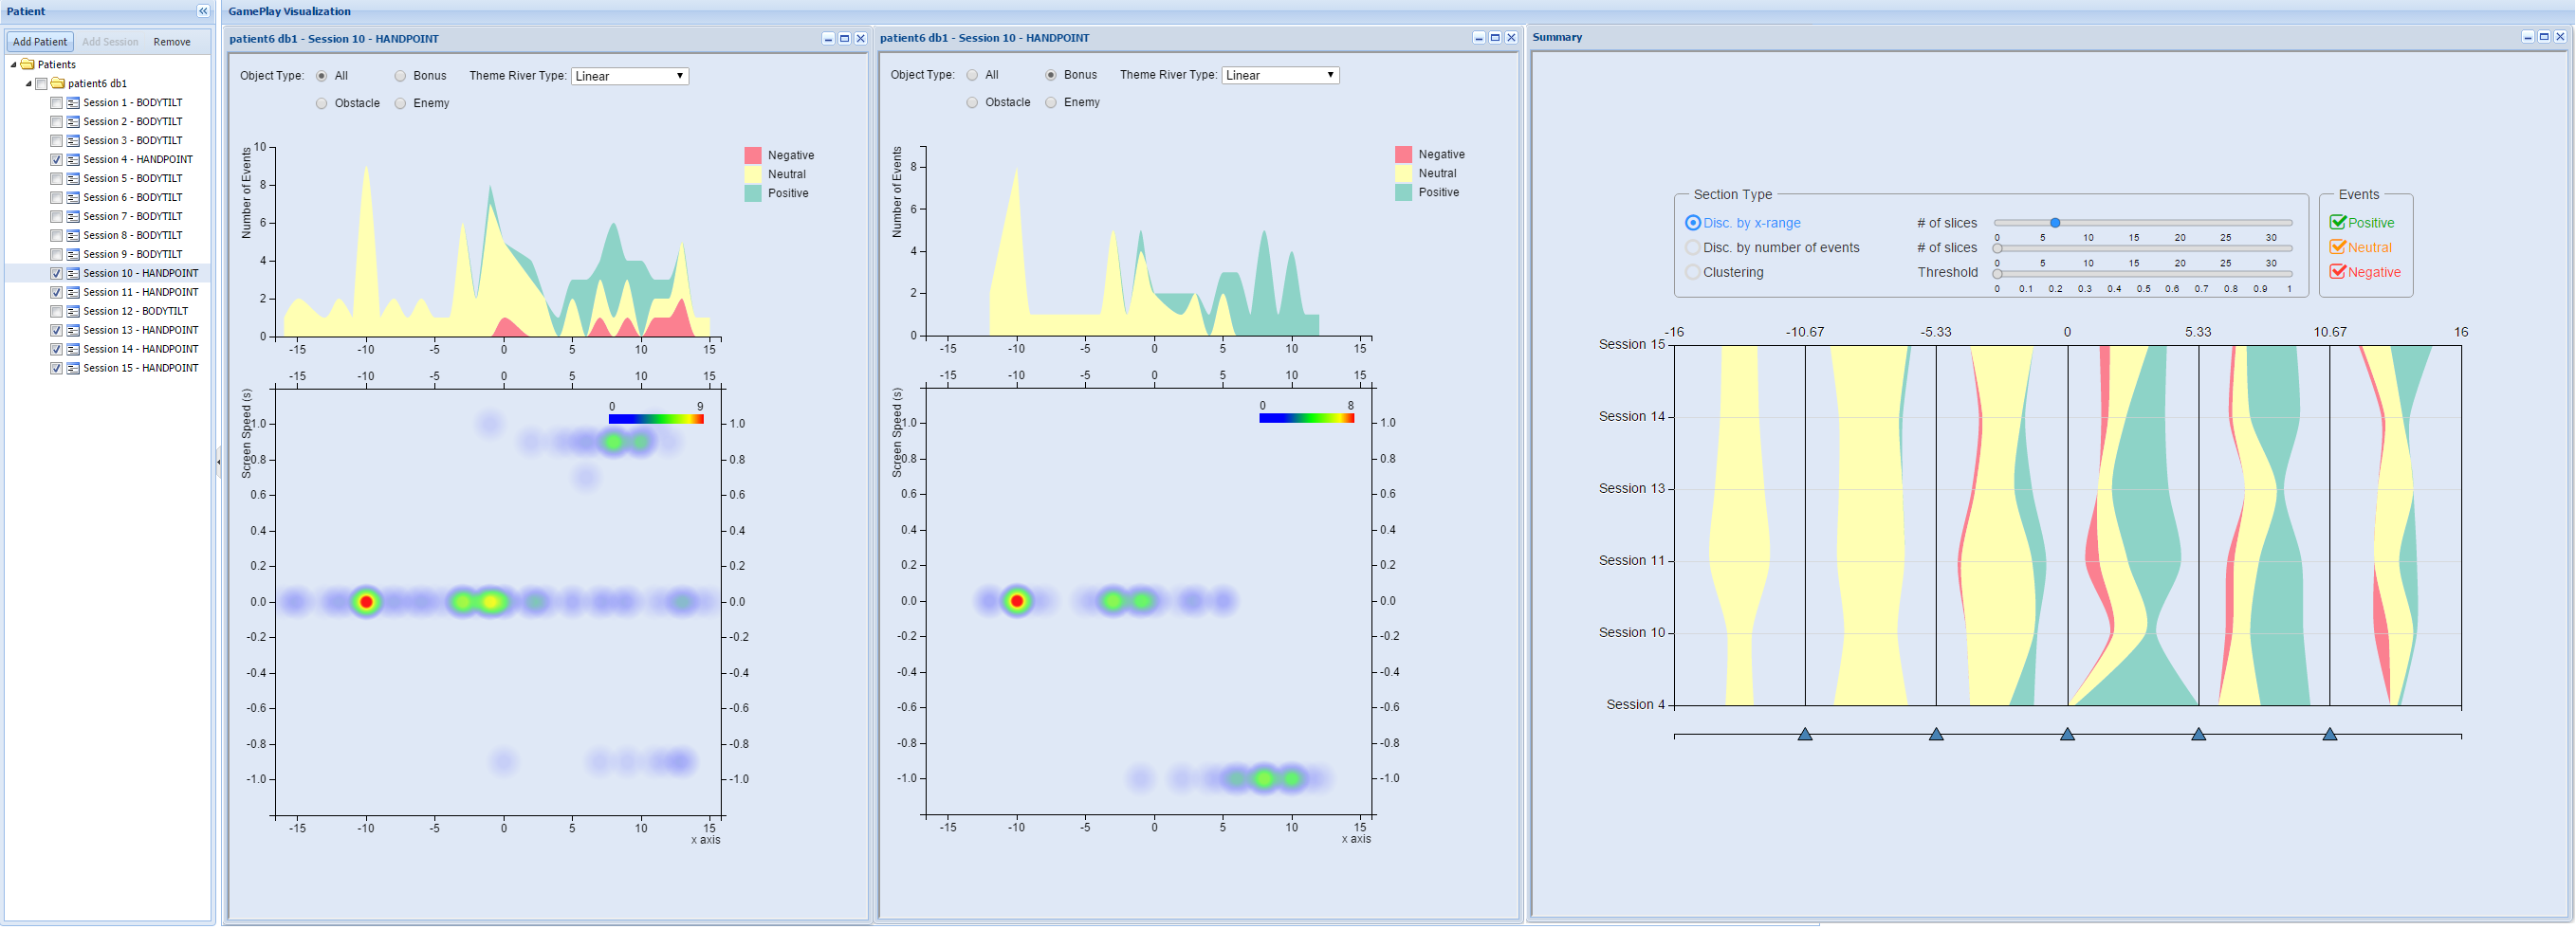
\includegraphics[width=180mm]{images/interface_all3.png}
	\caption{The general interface of the visualization is divided into: (i) Navigation area (left) where user can choose players and sessions. (ii) Visualization area (right) where the user can see the visualization. The windows on the left and middle are Session Visualization which show movement on one session. The window on the right is Summary Visualization which shows movement evolution overtime.}
	\label{fig:interface_all}
\end{figure*}

\subsection{Session Visualization}
The Session Visualization shows events within a game session. The requirement can be split into two: (i) knowing the distribution of events and movements (ii) knowing the distribution of events, movements and screen speed. Basically, (ii) is a detailed view of (i). Therefore, there are two chart developed to meet these requirements: stacked area graph for (i) and heatmap for (ii), each of which will be explained in details in this subsection.

\subsubsection{Stacked Graph}
Build on layered area graph, Stacked Graph is widely used to visualize evolution of variable over times such as document theme \cite{havre}, box office movie revenue\footnote{\url{http://www.nytimes.com/interactive/2008/02/23/movies/20080223_REVENUE_GRAPHIC.html?_r=0}}, listening history in Last.fm \cite{byron}, etc. Stacked Graph is chosen because its ability to show individual value of a variable, the difference between values of different variables as well as the total of overall value. In our approach, instead of using this metaphor to show evolution over time, it is used to show distribution of events over spatial coordinate \ref{t11} as shown in Figure \ref{fig:interface_all} (top middle). Here, the horizontal axis represents x coordinate and vertical axis represents number of events. Each event category is represented as an area with different color: Red (Negative), Yellow (Neutral), and Green (Positive). However, with this approach it is difficult to see the trend for each individual events which is not on the base of the chart. \cite{alan} propose an interactive solution to this problem by sinking the selected category to the horizontal axis. Thus, in our visualization, different layout of stacked graph is provided: (1) Linear (Figure \ref{fig:interface_all} middle): zero y axis is used as the baseline, with the stack ordered from the bottom as Negative, Neutral, Positive. (2) Silhouette (Figure \ref{fig:layout} top left): the graph is centered as in streamgraphs. (3) Positive (Figure \ref{fig:layout} top right): zero y axis is located at the top of the chart and is used as the baseline with the stack ordered from the top as Positive, Neutral, Negative. (4) Neutral-Negative (Figure \ref{fig:layout} bottom right): zero y axis is located in the middle of the chart. Neutral and Positive events are shown on the positive area of y axis and Negative events are shown on the negative area of y axis. (5) Positive-Neutral (Figure \ref{fig:layout} bottom left): zero y axis is located in the middle of the chart. Positive events are shown on the positive area of y axis, while Neutral and Negative events are shown on the negative area of y axis.
\begin{figure}
	\centering
	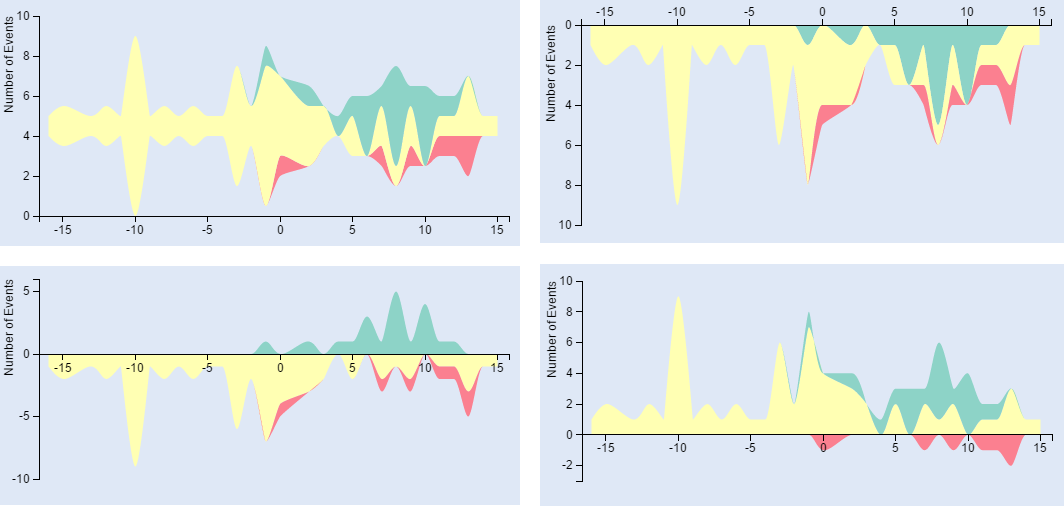
\includegraphics[width=85mm]{images/layout.png}
	\caption{Stacked Graph Layout: Silhouette (top left), Positive (top right), Positive-Neutral (bottom left), Neutral-Negative (bottom right)}
	\label{fig:layout}
\end{figure}
For each stacked graph layout, user can choose which object type to show on the graph \ref{t13}. Options are available as radio button on top of the chart. Therefore, choosing Bonus will show only Positive and Neutral events, choosing Obstacle will show only Neutral and Negative events, and choosing Enemy will show all event type.

\subsubsection{Heat Map}

Heat Map is a quite popular visualization method nowadays due to its ability which allows user to see variable with the highest value at one glance. Most of the time, heatmap is implemented on geographical map to represent variable value over certain area on map, i.e: Natural Disaster Risk by Location\footnote{\url{http://www.rms.com/}}, population density\footnote{\url{https://en.wikipedia.org/wiki/Population_density}}, Number of picture taken in an area\footnote{\url{http://sightsmap.com/}}, etc. Heat map is also used to track eye movement or mouse click on a website, and representing DNA microarray data in the form of cluster heat map \cite{friendly}. Heat map uses color gradation to represent the hotness level of a variable. Usually, red color is used to represent the high value (hot) and blue is used to represent the low value (cold). However, other color combination can also be used. To represent distribution of events and screen speed over x axis \ref{t12}, the events are first grouped based on their x values and normalized screen speed. The number of events is then represented as heat map on the graph with highest number of events in red color and the lowest number of events in blue color. Normalized screen speed is represented as vertical axis and x value is represented as horizontal axis. Each event category is presented in different heatmap area: top for Positive, middle for Neutral, and bottom for Negative (Figure \ref{fig:interface_all} bottom middle). For Neutral events, the screen speed is not calculated since it basically means an object has been avoided or missed. For Negative events, the screen speed is represented in negative to show that it's an uncalculated movement. For the heatmap, user can also choose to show a specific object \ref{t14} by clicking the radio button associated with the desired object. 

\subsection{Summary Visualization}
\begin{figure*}
	\centering
	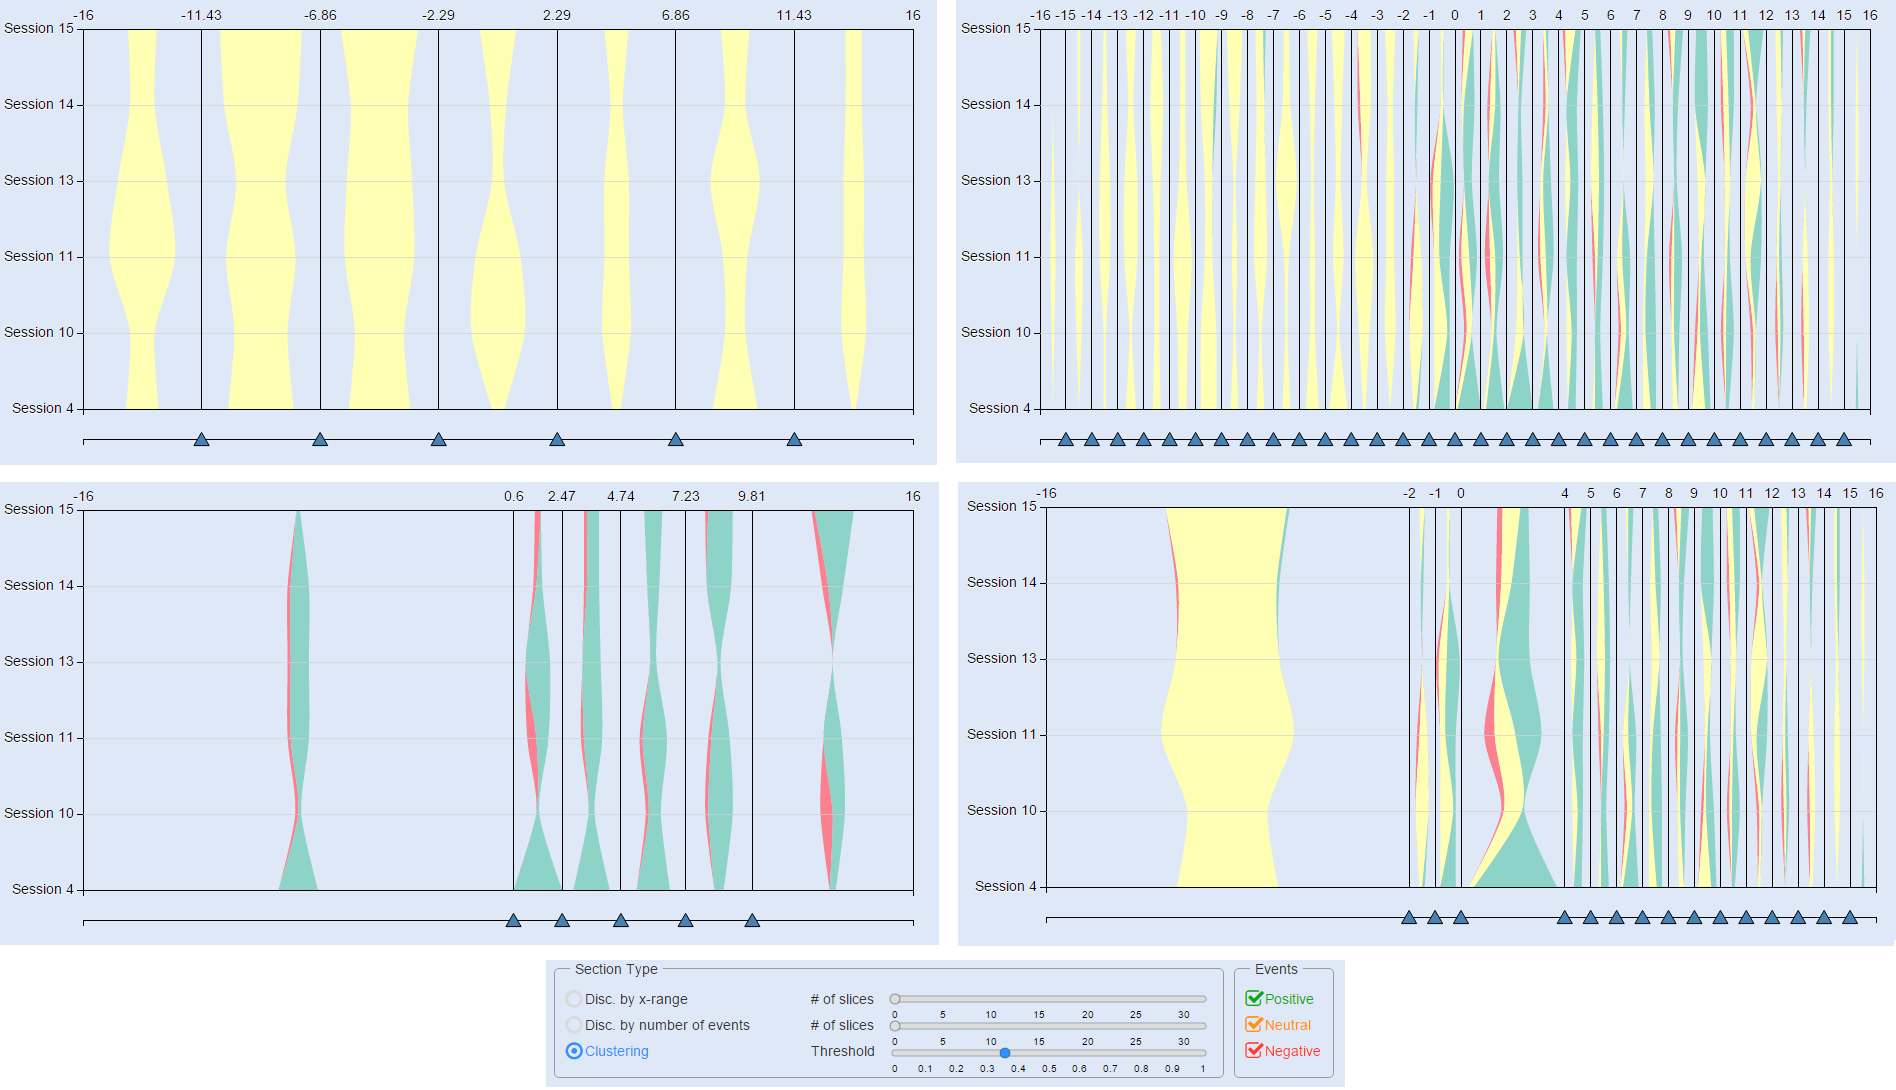
\includegraphics[width=180mm]{images/case_study_all2.png}
	\caption{Summary Visualization divided by x-range filtered with Neutral events (top left), divided by total number of Positive and Negative events (middle left), clustered with threshold=0 (top right), clustered with threshold=0.35 (middle right), and navigation bar (bottom)}
	\label{fig:case_study_all}
\end{figure*}
The Summary Visualization fulfills the requirements concerning movement evolution over time (\textit{T}2.x). In this case, a single session is considered as a single time point. Since user are interested in evolution over a certain x-area, the visualization are divided into sections of x-area. There are three ways of division: by the range of x-area, by the number of events within an area, and by clustering. The following explains the three approaches and its interaction technique in details.

\subsubsection{Visualization by range of x-area}
To fulfill \ref{t21}, a streamgraph metaphor is chosen to show evolution of movement (represented by events) over time. Time is often displayed on x-axis, but here, x-axis represent the x-axis of the screen, so time is displayed on the y-axis. Some visualizations are also based on this approach, like Visual Sedimentation \cite{huron}. Here, sessions represent time with the earliest one shown at the bottom and the latest one shown on the top. The x axis is then divided into sections of the same range based on user input. For each section, events are then filtered to the one which happened within the section x boundary. The filtered events are grouped based on session number and event category. Number of events within this group is then presented in vertical streamgraph layout with event type represented using the same color used in the Session visualization (Figure  \ref{fig:interface_all} right). For each section, it is possible to see which session has the most or least number of events by comparing the total length of all event category in one session. 

\subsubsection{Visualization by number of events}
This second type of Summary Visualization uses the same approach explained previously. However, a section is calculated based on the total number of positive and negative events instead of the range of x-axis \ref{t23}. Therefore, based on the distribution of positive and negative events, one section in the chart may have bigger x-range than the other section. Only by comparing the size of sections, it's possible to know in which area most of the events are concentrated. Figure \ref{fig:case_study_all} (middle left) shows that the events are more concentrated in the right area of the screen. 

\subsubsection{Visualization by clustering}
This third type of visualization fulfills \ref{t25}. As explained in section 4.2, initially the chart is divided into sections with range equals to an x-axis unit. Depending on the threshold value inputted by user, consecutive sections with distance below the threshold will be merged. This process is repeated until there is no sections with distance below the threshold. The input threshold ranges from 0 to 1. Thus, when user inputted threshold = 0, none of the section will be merged. On the other hand, when user inputted threshold = 1, all of the sections will be merged. Figure \ref{fig:case_study_all} top right shows when user input threshold = 0, while Figure \ref{fig:case_study_all} middle right shows threshold = 0.35. As we can see, there are some sections which are merged, indicated with bigger section size. 

\subsubsection{Interaction Technique}
On top of the chart, an interaction bar is provided where user can interact with and change some variable in the chart. In first panel of the interaction bar (Figure \ref{fig:case_study_all} bottom), three sliders are provided: (i) slider to input the number of slices so that each section will have the same x-range (ii) slider to input the number of slices so that each section will have the same total number of positive and negative events (iii) slider to input threshold so that each section will have a cluster of similar movement evolution. When user uses slider (i) and (ii), the value on the slider defines the number of sections on the chart. For (i), the more number of sections, the smaller the x-range. While for (ii), the value selected on the slider is a denominator. The input is calculated by dividing total number of all positive and negative events by the value selected on the slider. Thus, the smaller the number chosen on the slider, the bigger the number of events. In the second panel, user has the options to choose which event type to show on the chart. This fulfills requirement \ref{t22} and \ref{t24}. By default all event type will be shown. 

Once the chart is generated, user has the ability to slide/drag the line between each session or the small triangle at the bottom of the line to the right or left to change the range of it's neighbouring sections \ref{t21}\ref{t23}. While dragging, the text on top of the line changes based on the current x value of the dragged line. When a line is dragged over another line, the two sections will be merged creating a new section with different x range. Therefore, user may be able to gain the information in which particular area a certain type of events starting to happened. It is also possible to divide a section into two sections by clicking the top area of the chart in between the lower and upper section boundary text. This allows user to know the distribution of event type within a section.

\subsection{General Interface}

Both the Session and Summary visualization are attached into an application which allows user to navigate different player and session. Unlike the visualization interface which uses d3.js and heatmap.js library, the general interface is built using extjs library which allows the development of desktop-like web application. The interface of this application is divided into two areas: Navigation area and Visualization area (Figure \ref{fig:interface_all}). In Navigation area, user can choose patient and the sessions they have played. On clicking a session, a Session visualization of this session will be shown on the visualization area. It is also possible to open more than one Session visualization and rearrange the visualization window to compare gameplay between sessions (similar to navigating multiple windows in desktop). On clicking patient's name, Summary visualization for the chosen session will be shown.

\section{Case Study}

To evaluate the visualization functionality developed in this thesis, a case study will be presented. In this case study we use data set from games played by patients. These data set are collected by NaturalPad. Unfortunately, it is not possible to get information concerning patients' pathology due to confidentiality reason. 

We have several patient data sets, however most of these data sets have very small number of session. Thus for this case study, we chose data sets from patient with enough sessions so that we can confirm the functionality of the developed visualization interface. Consequently, we chose data sets with 15 sessions which are played over the course of three weeks. These sessions are of two game type: HANDPOINT (6 sessions) and BODYTILT (9 session). Here, only the sessions of HANDPOINT exercise will be discussed. 

Focusing on the second session of HANDPOINT shown in Figure \ref{fig:interface_all} (left window) stacked graph, it can be seen that the positive and negative events only appear on the right half of the chart indicating that the player only move to the right \ref{t11}. The yellow area are bigger compared to the green and red areas, showing that there are a lot of missed/avoided objects. 

From Figure \ref{fig:interface_all} (left window) heatmap, we can see that there are many Neutral events on the left side of the screen. While Positive and Negative events are happened only on the right side with similar screen speed indicating that the player didn't change the pace of the game \ref{t12}. Figure \ref{fig:interface_all} (middle window) shows events related to bonus \ref{t13}\ref{t14}. Therefore, there are only Positive and Neutral events. Here, it can be seen that on the far right, there are no bonus missed, however, on the left side all bonuses are missed. Based on these charts, we may conclude that the player has some difficulty to move to the left. It's important to see if this is an isolated case or happened all the time. Therefore, we need to see the pattern of movement for all sessions which will be discussed shortly.

The summary visualization shown in Figure \ref{fig:interface_all} (right window) confirmed that for 4 sessions, the player only move to the right side. However, from the fifth sessions, there are movements on the left side indicated by a small number of negative and positive events \ref{t21}. Figure \ref{fig:case_study_all} top left shows the evolution of neutral events \ref{t22}. Here, we can see that there are more neutral events on the left side compared to the right throughout all sessions. In Figure \ref{fig:case_study_all} top right, we can see that four sections between 0 and 4 have similar neutral event evolution. Hence, the sections are merged together forming one section \ref{t25} (see Figure \ref{fig:case_study_all} middle right). Consistent with all the previous visualization, Figure \ref{fig:case_study_all} middle left shows that the movements are concentrated more on the right side [\ref{t23}\ref{t24}].

On this case study, throughout all sessions the movements are concentrated to the right side with almost no movement on the left side. Therefore we can assume that the patient has his left side of the body affected. 

\section{Conclusion}

In this paper we presented a visualization interface to help healthcare professionals analyse gameplay of Hammer and Planks, a serious game which is used to rehabilitate patient with balance disorder. Player movement, represented by events happened in the game world, are visualized in two type of views: (i) \textit{Session Visualization} which allows user to analyse movement in one session. (ii) \textit{Summary Visualization} which allows user to analyse movement evolution over several sessions. For this visualization, a clustering algorithm based on hierarchical clustering to aggregate similar movement patterns over consecutive sections is introduced. Here, we proposed a new similarity measure for time series data. Even though the clustering algorithm presented here is applied to a specific time-series data, it can also be applied to other time-series data with different variables. Using the same abstraction, rows on the matrix represents time and columns represent different variables of the data set.

To evaluate the interface functionality, a case study from game played by patient is presented. The discussed case is able to show the effectiveness of the interface in achieving the tasks defined and therefore help the healthcare professionals assessing the progress of rehabilitation.

We identified some limitations in our research that could be improved in future work. First, the distance function used in the clustering algorithm is based on euclidean distance. Although currently this distance function are able to quantify the difference in events proportion and evolution, it will be interesting to investigate other distance function and to see if it can improve the clustering. Another limitation is the data set used in the case studies isn't accompanied with pathology information. It will be interesting to study different type of pathology and it's movement pattern. In the future, these data can be used to improve the game by proposing game setting based on the type and severity of pathology. Lastly, current interface only explore log data related to events. Log data related to skeleton movement of the players throughout the game hasn't been explore. For future work, an interface visualizing the body movement and identifying different kind of movement quality and quantity (repetition, smoothness, accuracy, etc.) can help healthcare professional to improve the quality of rehabilitation process. 

%% if specified like this the section will be ommitted in review mode
%\acknowledgements{
%The authors wish to thank A, B, C. This work was supported in part by
%a grant from XYZ.}

\bibliographystyle{abbrv}
%%use following if all content of bibtex file should be shown
%\nocite{*}
\bibliography{template}
\end{document}
